\documentclass[11pt]{article}
\usepackage[margin=2.7cm]{geometry}
\usepackage[T1]{fontenc}
\usepackage[utf8]{inputenc}
\usepackage{lmodern,amsmath,amssymb,amsthm,tikz}
\usepackage[hidelinks]{hyperref}
\newtheorem{theorem}{Theorem}
\theoremstyle{remark}\newtheorem*{remark}{Remark}
\newcommand{\Z}{\mathbb{Z}}
\title{Symmetric exclusion on two half-spaces of $\Z^3$:\\ a non-reversible stationary measure}
\author{counterexamples-ips, entry 0002}
\date{Status: \emph{plausible} (not yet checked by a human)\\[2pt]\small Counterexample: ChatGPT Astra-6 (Section 8 of the manuscript in \texttt{raw/})\\ Digest: Claude (Opus 5.5), 2 November 2026}
\begin{document}
\maketitle

\paragraph{Question.} For exchange dynamics on a connected graph of bounded degree, with positive rates on every edge: is every stationary measure with finite energy reversible? On recurrent graphs (in particular $\Z^d$, $d\le2$) the answer is \emph{yes}, by the conservative analogue of Holley--Stroock (Section~7 of the source). On transient graphs the answer is \emph{no}.

\paragraph{Setting.} Let $H_+=\{x\in\Z^3:x_1\ge1\}$, $H_-=\{x\in\Z^3:x_1\le0\}$, $o_-=(0,0,0)$, $o_+=(1,0,0)$. The graph $G$ on $\Z^3$ has as edges all nearest-neighbour bonds inside $H_+$ or inside $H_-$, and the single bridge $\{o_-,o_+\}$.

\begin{center}
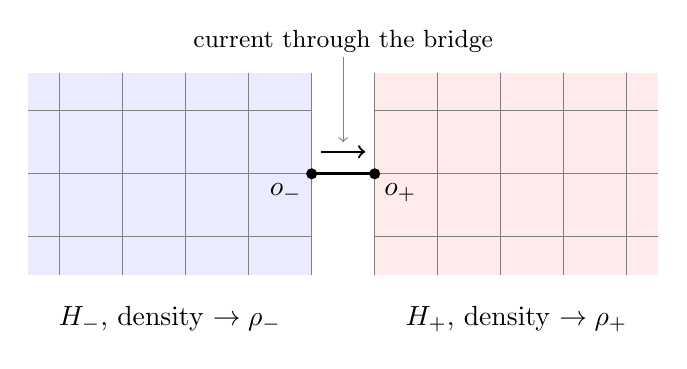
\begin{tikzpicture}[scale=0.8]
\fill[blue!8] (-5,-1.6) rectangle (-0.5,1.6); \fill[red!8] (0.5,-1.6) rectangle (5,1.6);
\foreach \y in {-1,0,1}{\draw[gray] (-5,\y)--(-0.5,\y); \draw[gray] (0.5,\y)--(5,\y);}
\foreach \x in {-4.5,-3.5,-2.5,-1.5,-0.5}{\draw[gray] (\x,-1.6)--(\x,1.6);}
\foreach \x in {0.5,1.5,2.5,3.5,4.5}{\draw[gray] (\x,-1.6)--(\x,1.6);}
\draw[very thick] (-0.5,0)--(0.5,0);
\fill (-0.5,0) circle (2.5pt) node[below left] {$o_-$}; \fill (0.5,0) circle (2.5pt) node[below right] {$o_+$};
\node at (-2.75,-2.3) {$H_-$, density $\to\rho_-$}; \node at (2.75,-2.3) {$H_+$, density $\to\rho_+$};
\draw[->,thick] (-0.35,0.35)--(0.35,0.35); \node[fill=white,inner sep=1pt] at (0,2.1) {\small current through the bridge}; \draw[gray,->] (0,1.85)--(0,0.5);
\end{tikzpicture}
\end{center}

SEP on $G$ exchanges the spins at the endpoints of each edge of $G$ at rate $1$. A measure is reversible iff it is invariant under each exchange $\theta_b$, $b$ an edge of $G$; all Bernoulli product measures $\nu_\rho$ are reversible.

\begin{theorem}[Theorem 8.1 of the source]
Let $0<\rho_-<\rho_+<1$. SEP on $G$ has a stationary measure $\mu^*$ that is not reversible and has finite energy with constant $\delta=\min\{\rho_-,1-\rho_+\}$. Moreover $\mu^*(\eta_x=+1)\to\rho_\pm$ as $|x|\to\infty$ in $H_\pm$.
\end{theorem}

\begin{proof}[Proof (summary)]
\emph{Step 1.} Simple random walk $X$ on $G$ is transient (fold $\Z^3$ along $\{x_1=\frac12\}$; Rayleigh monotonicity), so it crosses the bridge finitely often, and\[\alpha(x):=P_x(X\text{ eventually stays in }H_+)\]is harmonic with $0\le\alpha\le1$. By the reflection symmetry $\alpha(1-x_1,x_2,x_3)=1-\alpha(x)$, and $\alpha>\frac12$ far out in $H_+$; so $\alpha$ is not constant. Put $\beta=\rho_-+(\rho_+-\rho_-)\alpha$.

\emph{Step 2.} Start from the product measure $\nu_\beta$. The one-point function $u_t(x)$ of SEP solves $\partial_t u=\Delta_G u$; since $\beta$ is harmonic, $u_t=\beta$ for all $t$.

\emph{Step 3.} A weak limit $\mu^*$ of Ces\`aro averages of $\nu_\beta T_t$ is stationary, with $\mu^*(\eta_x=+1)=\beta(x)$.

\emph{Step 4.} Reversibility would force $\beta(x)=\beta(y)$ along every edge, so $\beta$ would be constant on the connected graph $G$.

\emph{Step 5.} By the stirring construction $\eta_t=\eta_0\circ\pi_t^{-1}$ with $\pi_t$ independent of $\eta_0$; conditionally on $\pi_t$ the spins are independent with densities in $[\rho_-,\rho_+]$, which gives finite energy.
\end{proof}

\paragraph{Mechanism.} The half-spaces act as two reservoirs at densities $\rho_-$ and $\rho_+$ joined by one wire. Because they are transient, particles that cross the bridge wander off rather than equilibrating the two sides, so the density difference persists and a current flows through the bridge in the stationary state. A current is incompatible with reversibility. On recurrent graphs bounded harmonic functions are constant and every stationary measure of SEP is a mixture of Bernoulli measures (Liggett's characterisation).

\begin{remark}[Interacting version, Theorem 8.3 of the source; not checked]
For exchange rates on $G$ associated with a potential $J$ with $\sum_F|J_F|<\infty$, there is a reversible measure ($\propto e^{-\Phi}\nu_\rho$) and also a stationary measure $\mu$ with $|\mu(\eta_x=+1)-\beta(x)|\le\gamma(x)\to0$, hence not reversible. Proof by coupling with SEP. Whether $\mu$ has finite energy is open.
\end{remark}

\paragraph{Which hypothesis breaks.}
(i) $G$ is not $\Z^3$: rates vanish on all bonds crossing $\{x_1=\frac12\}$ except one. With rates bounded away from $0$ on all bonds of $\Z^3$, bounded harmonic functions are constant (elliptic Harnack) and all stationary measures of SEP are reversible.
(ii) The dynamics is conservative; for spin flips no analogue is known, so the Holley--Stroock question in $d\ge3$ remains open.
(iii) The example shows that recurrence cannot be dropped from the graph version of the conservative Holley--Stroock theorem.

\paragraph{Follow-up questions.} See \texttt{entries/0002-sep-two-half-spaces-z3/followups.md}.

\begin{thebibliography}{9}\small
\bibitem{HS77} R.~Holley, D.~Stroock, In one and two dimensions, every stationary measure for a stochastic Ising model is a Gibbs state, \emph{Comm.\ Math.\ Phys.}\ 55 (1977).
\bibitem{Li73} T.~M.~Liggett, A characterization of the invariant measures for an infinite particle system with interactions, \emph{Trans.\ Amer.\ Math.\ Soc.}\ 179 (1973); II, \emph{ibid.}\ 198 (1974).
\bibitem{Li85} T.~M.~Liggett, \emph{Interacting Particle Systems}, Springer, 1985, Ch.~VIII.
\bibitem{LP16} R.~Lyons, Y.~Peres, \emph{Probability on Trees and Networks}, CUP, 2016, Ch.~2.
\bibitem{LT24} P.~Lammers, F.~L.~Toninelli, Non-reversible stationary states for majority voter and Ising dynamics on trees, \emph{Electron.\ J.\ Probab.}\ 29 (2024).
\end{thebibliography}
\end{document}
